\documentclass[10.5pt,notitlepage]{article}
\usepackage[utf8]{inputenc}
\usepackage{amsthm}
\usepackage{amsmath}
\usepackage{amsfonts}
\usepackage{mathtools}
\usepackage{amsmath,amssymb}       
\usepackage{enumitem}   
\usepackage{enumerate}
\usepackage{verbatim} 
\usepackage{bbm}
\usepackage{hyperref}
\usepackage{booktabs}
\renewcommand{\qedsymbol}{$\blacksquare$}
\usepackage{makecell}
\usepackage[spanish]{babel}
\decimalpoint
\usepackage[letterpaper]{geometry}
\usepackage{mathrsfs}
\newenvironment{solucion}
  {\begin{proof}[Solución]}
  {\end{proof}}
\pagestyle{plain}
\usepackage{pdflscape}
\usepackage[table, dvipsnames]{xcolor}
\usepackage{longtable}
\usepackage{tikz}
\def\checkmark{\tikz\fill[scale=0.4](0,.35) -- (.25,0) -- (1,.7) -- (.25,.15) -- cycle;} 
\usepackage[bottom]{footmisc}
\usepackage{hyperref}
\usepackage{float}
\usepackage[utf8]{inputenc}
\usepackage{bbm}
\usepackage{placeins}
\newcommand{\pp}{\mathbb{P}}
\newcommand{\BB}{\mathcal{B}}
\newcommand{\RR}{\mathbb{R}}
\newcommand{\FF}{\mathcal{F}}
\newcommand{\CC}{\mathcal{C}}
\newcommand{\oo}{\varnothing}
\newcommand{\ee}{\varepsilon}
\newcommand{\NN}{\mathbb{N}}
\newcommand{\PP}{\mathcal{P}}
\newcommand{\LL}{\mathrm{L}}
\newcommand{\XX}{\mathbf{X}}
\newcommand{\xx}{\mathbf{x}}
\DeclareMathOperator{\Tr}{Tr}
\newcommand{\abs}[1]{\left\lvert #1 \right\rvert}
\newcommand{\norm}[1]{\left\| #1 \right\|}
\newcommand{\inner}[1]{\left\langle #1 \right\rangle}
\newcommand{\corch}[1]{\left[ #1 \right]}
\newcommand{\kis}[1]{\left\{ #1 \right\}}
\newcommand{\pare}[1]{\left( #1 \right)}

\theoremstyle{plain}

\newtheorem{thm}{Teorema}[section] % reset theorem numbering for each chapter
\newtheorem{defn}[thm]{Definición} % definition numbers are dependent on theorem numbers
\newtheorem{lem}[thm]{Lema} % same for example numbers
\newtheorem{remarkex}{Observación}
\newenvironment{rem}
  {\pushQED{\qed}\renewcommand{\qedsymbol}{$\triangle$}\remarkex}
  {\popQED\endremarkex}

\usepackage{geometry}
\usepackage{mathtools}
\usepackage{enumitem}
\usepackage{framed}
\usepackage{amsthm}
\usepackage{thmtools}
\usepackage{etoolbox}
\usepackage{fancybox}

\newenvironment{myleftbar}{%
\def\FrameCommand{\hspace{0.6em}\vrule width 2pt\hspace{0.6em}}%
\MakeFramed{\advance\hsize-\width \FrameRestore}}%
{\endMakeFramed}
\declaretheoremstyle[
spaceabove=6pt,
spacebelow=6pt
headfont=\normalfont\bfseries,
headpunct={} ,
headformat={\cornersize*{2pt}\ovalbox{\NAME~\NUMBER\ifstrequal{\NOTE}{}{\relax}{\NOTE}:}},
bodyfont=\normalfont,
]{exobreak}

\declaretheorem[style=exobreak, name=Ejercicio,%
postheadhook=\leavevmode\myleftbar, %
prefoothook = \endmyleftbar]{exo}
\usepackage{graphicx}
\graphicspath{ {images/} }
\title{Tarea 6: Modelos Estadísticos I.}

\author{Rojas Gutiérrez Rodolfo Emmanuel}

\begin{document}

\maketitle

\setcounter{exo}{0}
\begin{exo}[Ejercicio 1. Datos consumidores]
\end{exo}

\textbf{a) y b)}Primeramente observe en la figura \ref{fig1}
\begin{figure}[htb]
 \centering
 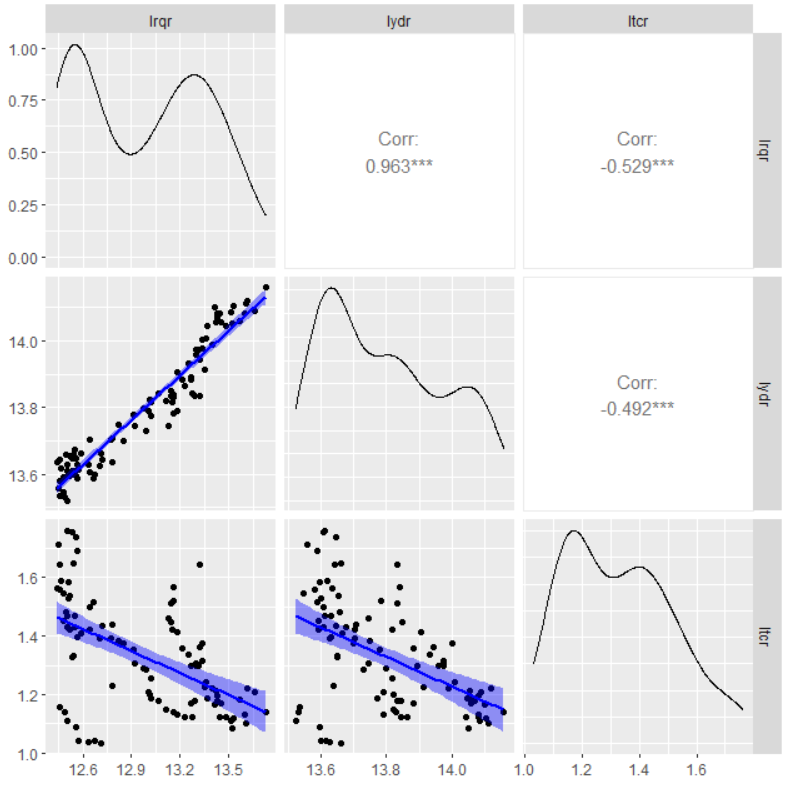
\includegraphics[scale = 0.65]{ExamenImG1.png}
 \caption{PairPlot con correlaciones de las variables independientes \(lrqr,lydr\) y \(ltcr\).}
\label{fig1}
\end{figure}
En ella podemos observar en parte superior las entradas por encima de la diagonal de la matriz de correlación entre las variables independientes, dado que las entradas en la diagonal son \(1\) y por la simetría de está matriz, esto es suficiente para determinar toda la matriz de correlación entre las variables independientes, note ahora que la correlación más alta es la existente entre las variables independientes \(lrqr\) y \(lydr\). Este hecho se ve reflejado en la parte inferior del gráfico donde es posible observar los gráficos de dispersión de las variables independientes con modelos de regresión lineal simple ajustados con sus respectivos intervalos de confianza. Note como el modelo para \(lrqr\) y \(lydr\) parece presentar una variabilidad casi inexistente en sus bandas de confianza, o que indica que una variable explica casi perfectamente a la otra. A partir de aquí se consideraron dos maneras de realizar los diagnósticos la primera es considerando la matriz \(\mathbf{X_{CE}}\) que es la matriz cuyas columnas corresponden a los valores de las variables independientes centrados y escalados, y \(\mathbf{X_{E}}\) que es la matriz cuyas columnas consideran un intercepto y a las variables independientes escaladas. Dado que la matriz de correlaciones de los datos no cambia si los centramos y escalamos, o solo los escalamos los \(VIF's\) para ambos casos resultan iguales y se presentan en la figura \ref{fig2}: 
\begin{figure}[htb]
 \centering
 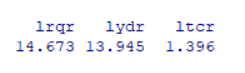
\includegraphics[scale = 0.80]{ExamenImG2.png}
 \caption{Vif's para los modelos de regresión.}
\label{fig2}
\end{figure}
Dado que los VIFS asociados a los coeficientes que pre-multiplican a las variables \(lrqr\) y \(lydr\) exceden el \(10\), se considera que estos coeficientes están siendo pobremente estimados debido a problemas de multicolinealidad. Por otro lado, se obtuvieron los números de condición de las matrices \(\mathbf{X_{CE}}' \mathbf{X_{CE}}\) y \(\mathbf{X_{E}}'\mathbf{X_{E}}\) los cuales se presentan en las figuras \eqref{fig3} y \ref{fig4} respectivamente 
\begin{equation}\label{fig3}
K(\mathbf{X_{CE}}' \mathbf{X_{CE}}) = 486325.2. 
\end{equation}
\begin{equation}\label{fig4}    K(\mathbf{X_{E}}' \mathbf{X_{E}}) =65.699.
\end{equation}
Llaman la atención dos cosas, en el modelo en que consideramos las columnas centradas y escaladas el número de condición es menor a \(100\) y por ende se considera que no existe un problema de multicolinealidad serio en este caso, sin embargo, el modelo que solo esta escalado tiene un número de condición por arriba de \(1000\) lo que indica un problema serio de multicolinealiadad. Esto no es de sorprender ya que al centrar y escalar las variables de respuesta recuerde que las variables independientes se vuelven ortogonales al intercepto, eliminando cualquier rastro de colinealiadad con este, por lo que se podría sospechar de la existencia de multicolinealidad con este. Dado que los VIFs en los modelos centrados y escalados arrojaron resultados alarmantes en ambos modelos, y debido a la fuerte relación lineal detectada entre las variables independientes \(lydr\) y \(lrqr\) se decidió que lo correcto sería quedarse con una y solo uno de estas variables independientes, de este modo para el modelo con variables independientes centradas y escaladas y variable respuesta centrada se obtuvieron los siguientes  resúmenes eliminando \(lydr\) y \(lrqr\): 
\begin{figure}[H]
 \centering
 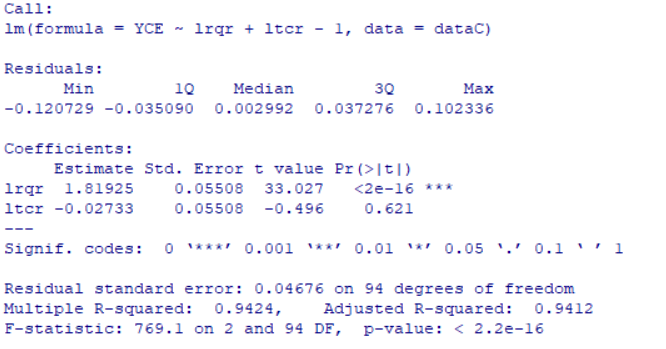
\includegraphics[scale = 0.80]{ExamenImG5.png}
 \caption{Resumen modelo con variables independientes centradas y escaladas y variable respuesta centrada. Eliminando la variable independiente \(lydr\).}
\label{fig5}

\end{figure}
\begin{figure}[H]
 \centering
 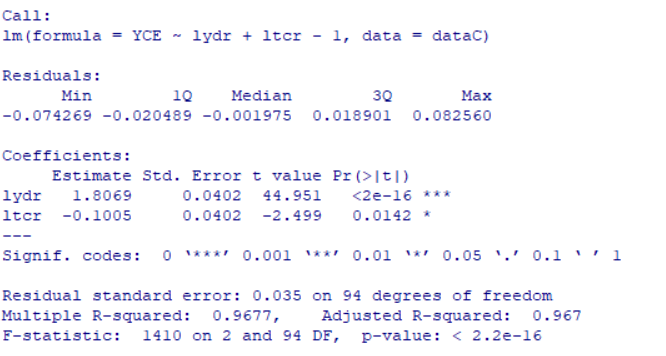
\includegraphics[scale = 0.80]{ExamenImG6.png}
 \caption{Resumen modelo con variables independientes centradas y escaladas y variable respuesta centrada. Eliminando la variable independiente \(lrqr\).}
\label{fig6}
\end{figure}
Observe que el modelo en el que se elimina a \(lrqr\) obtiene mejor \(R^2\), mejor \(R^2\) ajustada y sus dos coeficientes resultan significativos, por lo que, nos decantamos por este modelo. Los coeficientes en la escala original para el modelo en la figura \ref{fig6} se presentan en la figura \ref{fig7}.
\begin{figure}[htb]
 \centering
 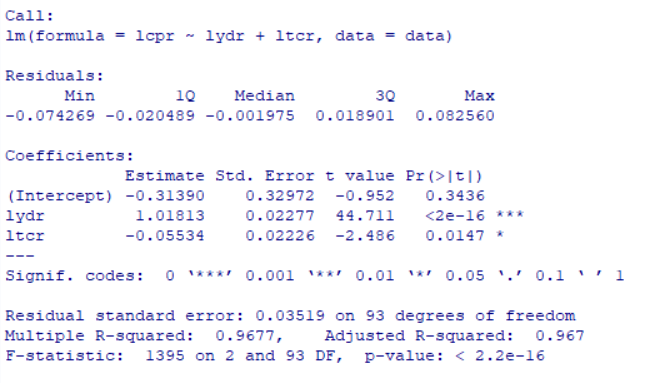
\includegraphics[scale = 0.80]{ExamenImG7.png}
 \caption{Resumen modelo con variables en escala original. Eliminando la variable independiente \(lrqr\).}
\label{fig7}
\end{figure}
Podemos ver que en este caso el intercepto no resulta significativo, de este modo se exploró la posibilidad de removerlo, (debido a los resultados obtenidos en el análisis que consideraba al intercepto y las variables solamente escaladas), lo cual arrojo el resumen presentado en la \ref{fig8}. Sorprende lo bueno de que resulta este modelo ya que alcanza un \(R^2\) y \(R^2\) ajustado de \(1\) y todos sus coeficientes resultan significativamente distintos de cero, bajo un nivel de significacnia del \(5\%\)
\begin{figure}[htb]
 \centering
 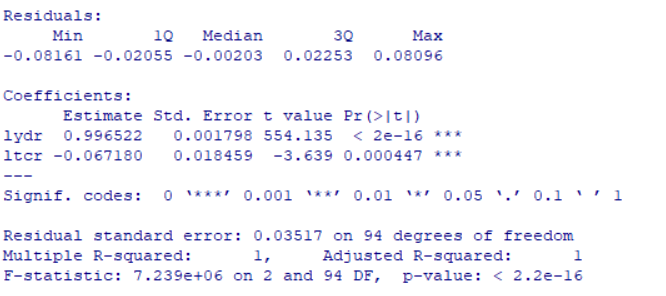
\includegraphics[scale = 0.80]{ExamenImG8.png}
 \caption{Resumen modelo con variables en escala original sin intercepto. Eliminando la variable independiente \(lrqr\).}
\label{fig8}
\end{figure}
Además la correlación entre \(lydr\) y \(lrqr\) es la más pequeña en valor absoluto entre todas las variables independientes, cosa que puede corroborarse en la figura \ref{fig1}, con un valor \(-0.492\), de este modo el los VIFS de este modelo, ambos son iguales a 
\begin{equation*}
    1/(1 - (-0.492)^2) \approx 1.319. 
\end{equation*}
Por lo que ningún parámetro esta siendo pobremente estimado debido a la multicolinealidad. \\ 

\noindent \textbf{c)}
Para \(i \in \kis{lqrq,\hdots,ltcr}\) se define el vector columna de datos \(X_i\) como aquel que resulta de centrar el vector columna \(i\) y posteriormente escalar el vector resultante dividiendo por su longitud.\footnote{Entiéndase por longitud su norma euclideana.} Sea ahora \(\mathbf{X_{CE}} = \begin{pmatrix}  X_{lrqr} & X_{lydr} & X_{ltcr}\end{pmatrix}\) 
ajustará\footnote{Note que \(\mathbf{X_{CE}}\) es exactamente la misma matriz que se definió en el inciso anterior} inicialmente el modelo
\begin{equation}\label{1.0}
 E[lpcr_{i}| X_{ilqrq}, \hdots, X_{iltcr}] =  \alpha + \delta_{1} X_{ilqrq} + \hdots+ \delta_{3} X_{iltcr}, \ i \in \kis{1, \hdots, 96}.
\end{equation}
 Sin embargo, de acuerdo a Hastie Tibsharani\footnote{Ver referencia 1, pp. 64.} considerando este modelo con las variables independientes centradas y escaladas se tiene que la estimación Ridge para el intercepto esta dada por \(\hat{\alpha} = \overline{lpcr} = 3.6568
\), y por ende es posible considerar de manera equivalente el modelo \eqref{1.2} y obtener mediante regresión Ridge las estimaciones para los coeficientes de dicho modelo utilizando la matriz de diseño \(\mathbf{X_{CE}}\)
\begin{equation}\label{1.2}
    E[lpcr_{i} - \overline{lpcr}| X_{ilqrq}, \hdots, X_{iltcr}] =  \delta_{1} X_{ilqrq} + \hdots+ \delta_{3} X_{iltcr}, \ i \in \kis{1, \hdots, 96}.
\end{equation}
 De este modo además se cumplirá una de las condiciones estipuladas en el artículo de Hoerl (1975), es decir que la matriz de diseño \(\mathbf{X_{CE}}\) estará escalada de tal suerte que \(\mathbf{X_{CE}}'\mathbf{X_{CE}}\) sea una matriz de correlación. Ahora, de acuerdo al artículo de Hoerl (1975) una manera de estimar el valor del parámetro de sesgo \(\mathit{k}\) que resulte óptimo\footnote{En el sentido de que este \(\mathit{k}\) sea tal que el error cuadrático promedio que comete el estimador Ridge sea el mínimo posible.} es \begin{equation*}
    \mathit{k_h} = \frac{p \hat{\sigma}^2}{\hat{\delta}' \hat{\delta}} = 0.001522308,
\end{equation*}
donde \(p\) es el número de parámetros en el modelo \eqref{1.2}, es decir \(p = 3\), \(\hat{\sigma}^2\) es una estimación de la varianza de los términos de error en el modelo \eqref{1.2}, la cual fue calculada usando la suma de cuadrados de los residuales del modelo \eqref{1.2} estimado por mínimos cuadrados y arrojó un valor de \(\hat{\sigma}^2 = 0.0009841351
\), y \(\hat{\delta}\) es el estimador de mínimos cuadrados para los coeficientes del modelo \eqref{1.2}.  Denote por \(\hat{\delta}_{(k_{h})}\) al vector de estimaciones Ridge de los coeficientes del modelo obtenido usando el parámetro de sesgo \(k_h\), calculado en el inciso \textbf{a)} de este ejercicio, entonces se tiene que
\begin{equation*}
    \hat{\delta}_{(k_{h})} = (\mathbf{X_{CE}}'\mathbf{X_{CE}} + k_h I_{p})^{-1}\mathbf{X_{CE}}'Y_{CE} =  \begin{pmatrix}  0.60119040\\
     1.24672385\\
   -0.05802807\end{pmatrix},
\end{equation*}
donde \(Y_{CE} = lpcr - \overline{lpcr} = \). De este modo los valores ajustados por este modelo pueden escribirse como:
\begin{equation*}
     E[lpcr_{i} - \overline{lpcr}| X_{ilqrq}, \hdots, X_{iltcr}] =  0.60119040X_{ilqrq} + \hdots+ -0.05802807 X_{iltcr}, \ i \in \kis{1, \hdots, 96}.
\end{equation*}
Para esto modelo se obtuvo un \(R^2\) de 
\begin{equation*}
    R^2 = 1 - SS(RES)/SS(TOT) =0.9743479. 
\end{equation*}
Este coeficiente de determinación es menor al \(R^2\) del modelo propuesto en el inciso anterior, y debido a que este modelo considera más parámetros se prefiere al modelo anterior. Además, el objetivo de la regresión Ridge no fue logrado, ya que en la figura \ref{fig999} podemos ver los factores de inflación de la varianza bajo este modelo a penas cambiaron, comparados con los dados al inicio de este ejercicio, con esta elección de \(k\) y dos de ellos siguen resultando mayores a \(5\)\\
\begin{figure}[htb]
 \centering
 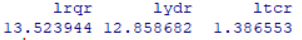
\includegraphics[scale = 0.80]{ExamenImG0.png}
 \caption{VIFS Modelo Ridge.}
\label{fig999}
\end{figure}

\textbf{d)} Por último, el resumen del modelo original sin ninguna escala esta dado en la figura \ref{fig9}
\begin{figure}[htb]
 \centering
 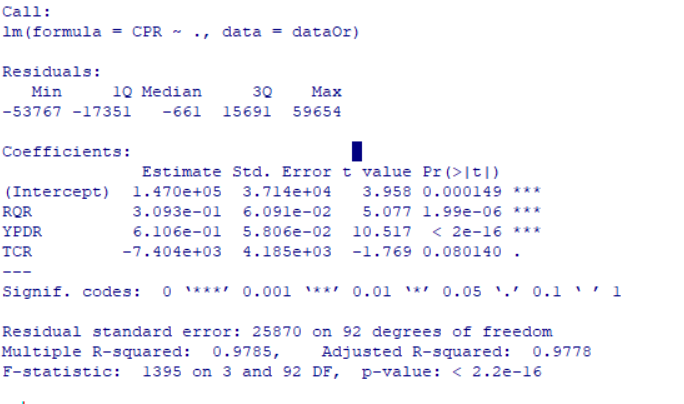
\includegraphics[scale = 0.80]{ExamenImG9.png}
 \caption{Resumen modelo con variables en escala original. Todas las variables}
\label{fig9}
\end{figure}
Se destaca que este modelo con todas las variables predictoras, no resulta mejor en \(R^2\) ni en \(R^2\) ajustada al mejor modelo presentado en los primeros dos incisos. 

\begin{exo}

\end{exo}
\begin{solucion}
\textbf{a) y b)} Primeramente observe en la figura \ref{fig11}
\begin{figure}[htb]
 \centering
 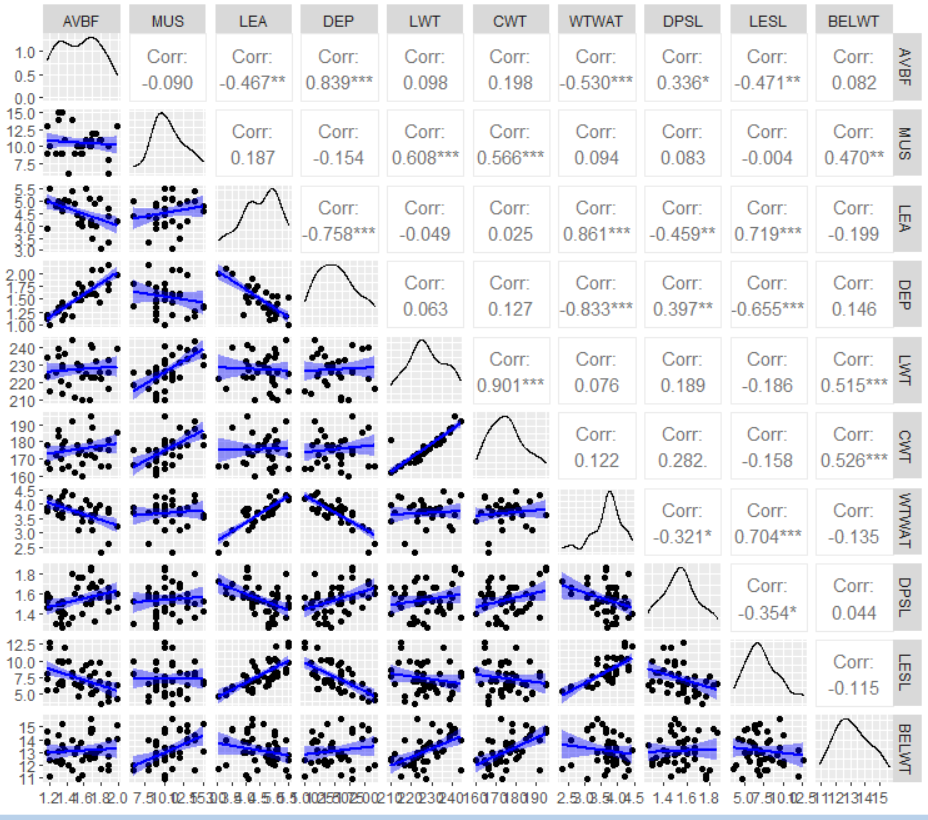
\includegraphics[scale = 0.65]{ExamenImG11.png}
 \caption{PairPlot con correlaciones de las \(10\) variables independientes.}
\label{fig11}
\end{figure}
En ella podemos observar en parte superior las entradas por encima de la diagonal de la matriz de correlación entre las variables independientes, dado que las entradas en la diagonal son \(1\) y por la simetría de está matriz, esto es suficiente para determinar toda la matriz de correlación entre las variables independientes, preocupan en especial la correlación existentes entre \(LWT\) y \(CWT\) con un valor de \(0.901\), la correlación existente entre \(LEA\) y \(WTWAT\) con un valor de \(0.861\) y la correlación existente entre \(DEP\) y \(WTWAT\) con un valor de \(-0.833\). En un segundo plano también llaman la atención las correlaciones entre \(LESL\) y \(DEP\) \(LESL\) y \(LEA\), por lo que, deberemos tener cuidado con estas variables. A partir de aquí se consideraron dos maneras de realizar los diagnósticos la primera es considerando la matriz \(\mathbf{X_{CE}}\) que es la matriz cuyas columnas corresponden a los valores de las variables independientes centrados y escalados, y \(\mathbf{X_{E}}\) que es la matriz cuyas columnas consideran un intercepto y a las variables independientes escaladas. Dado que la matriz de correlaciones de los datos no cambia si los centramos y escalamos, o solo los escalamos los \(VIF's\) para ambos casos resultan iguales y se presentan en la figura \ref{fig22}: 
\begin{figure}[htb]
 \centering
 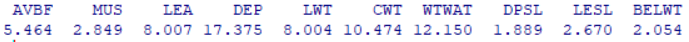
\includegraphics[scale = 0.80]{ExamenImG12.png}
 \caption{Vif's para los modelos de regresión.}
\label{fig22}
\end{figure}

Se observa que los VIFs asociados a los coeficientes que premultiplican a las variables \(AVBF\) y \(LWT\) exceden al 5, lo que da una primera alerta de que estos coeficientes pueden estar siendo pobremente estimados por problemas de multicolinealidad en el modelo, por otro lado, los coeficientes asociados  a las variables \(DEP, CWT\) y \(WTWAT\) exceden con claridad al \(10\), por lo que estos coeficientes si estan siendo pobremente estimados debido a la multicolinealidad. Note que varias de estas variables fueron mencionadas en el análisis de la matriz de correlaciones de las variables independientes. Por otro lado, se obtuvieron los números de condición de las matrices \(\mathbf{X_{CE}}' \mathbf{X_{CE}}\) y \(\mathbf{X_{E}}'\mathbf{X_{E}}\) los cuales se presentan en las figuras \eqref{fig33} y \ref{fig44} respectivamente 
\begin{equation}\label{fig33}
K(\mathbf{X_{CE}}' \mathbf{X_{CE}}) = 103834.9. 
\end{equation}
\begin{equation}\label{fig44}    K(\mathbf{X_{E}}' \mathbf{X_{E}}) =130.386.
\end{equation}
Llaman la atención dos cosas, en el modelo en que consideramos las columnas centradas y escaladas el número de condición se encuentra entre \(100\) y \(1000\) por ende se considera la multicolinealidad existente en el modelo es moderada, sin embargo, el modelo que solo esta escalado tiene un número de condición por arriba de \(1000\) lo que indica un problema serio de multicolinealiadad. Esto no es de sorprender ya que al centrar y escalar las variables de respuesta recuerde que las variables independientes se vuelven ortogonales al intercepto, eliminando cualquier rastro de colinealiadad con este, por lo que se podría sospechar de la existencia de multicolinealidad con dicho término de intercepto. De este modo, se tiene que las variables \(LWT\) y \(CWT\) estan fuertemente correlacionadas, por lo que se debería considerar quedarnos con una de ellas únicamente, dado que \(CWT\) posee el mayor factor de inflación de la varianza nos quedaremos con \(LWT\), por otro lado, todo el conjunto de variables independientes en el conjunto \(\kis{LEA, WTWAT, LESL,DEP}\) parecen tener problemas de colinealidad, ya que las correlaciones de todas estas variables resultan ser bastante elevadas, sin embargo, observando la figura \ref{fig22} se uno puede notar fácilmente que los factores de inflación de la varianza de \(DEP\) y \(WTWAT\) resultan ser los mas grandes en todo el conjunto de datos, por lo que se decidió eliminar igualmente estas variables. \footnote{Si da tiempo, se presentará la tabla de descomposición de varianzas para este problema en el anexo.}\\

\noindent \textbf{c)} Consideramos primeramente el modelo con las variables independientes centradas y escaladas y la variable respuesta centrada, en el que se removieron como ya se mencionó anteriormente las variables independientes en el conjunto \(\kis{CWT,DEP, WTWAT}\), las estimaciones así como un resumen para este modelo se consideran en la figura \ref{fig55}
\begin{figure}[htb]
 \centering
 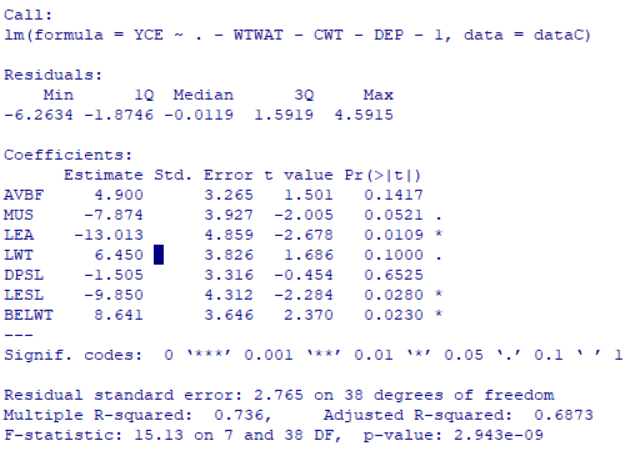
\includegraphics[scale = 0.80]{ExamenImG13.png}
 \caption{Resumen para modelo con las variables independientes centradas y escaladas y la variable respuesta centrada. Eliminado \(\kis{CWT,DEP, WTWAT}\).}
\label{fig55}
\end{figure}
Este mismo resumen pero con el modelo equivalente con los datos en las escalass originales se presenta en la figura \ref{fig66}
\begin{figure}[htb]
 \centering
 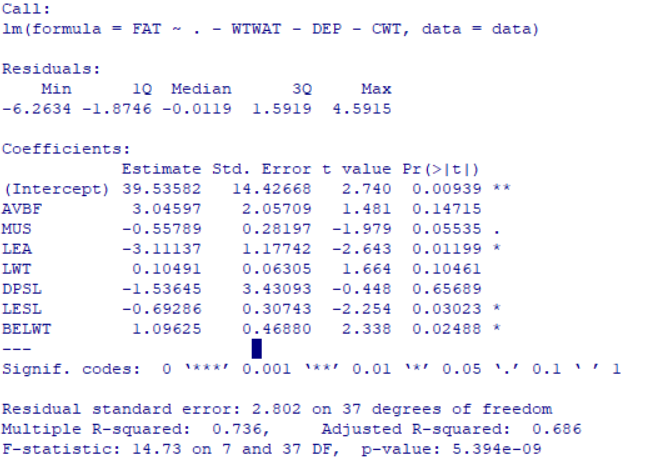
\includegraphics[scale = 0.80]{ExamenImG14.png}
 \caption{Resumen para modelo con las variables en la escala original. Eliminado \(\kis{CWT,DEP, WTWAT}\).}
\label{fig66}
\end{figure}
Luego por lo observado cuando se el análisis de la matriz de datos escalada en la que se considera la multicolinealidad con el intercepto, se decidió intentar ajustar el modelo anterior sin intercepto, a modo de analizar si la inclusión del mismo tenía efectos negativos por la posible multicolinealidad que este genera, lo que arrojó el análisis presentado en la figura \ref{fig77}. Puede verse que la significancia de varios coeficientes creció, además, en la última linea de la imagen presentada en la \ref{fig77} se presentan todos los factores de inflación de la varianza de los coeficientes de este modelo, observe que ninguno rebasa el \(5\), por lo que la multicolinealidad no es un problema para las estimaciones de los coeficientes en este modelo.
\begin{figure}[htb]
 \centering
 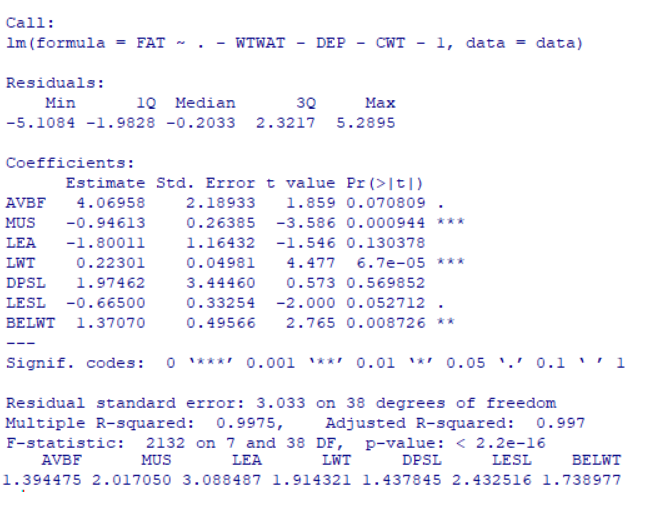
\includegraphics[scale = 0.80]{ExamenImG15.png}
 \caption{Resumen para modelo con las variables en la escala original. Eliminado \(\kis{CWT,DEP, WTWAT}\) y el término de intercepto.}
\label{fig77}
\end{figure}

Sin embargo, deseabamos encontrar un modelo con un mayor poder predictivo que el modelo original, y que además considerará el menor número de variables independientes en el, por lo cual, se decidió omitir las variables independientes \(DSPL\) y \(LEA\), las cuales no resultaban significativamente distintas de \(0\) bajo un nivel de significancia del \(5\%\) en el modelo presentado en la figura \ref{fig77}, obteniendo así el modelo presentado en la figura \ref{fig88}, en el mismo todos los coeficientes resultan significativamente distintos de cero y se tiene una \(R^2\) de \(0.9972\) y un \(R^2\) ajustada de \(0.9969\). Por último, los factores de inflación de la varianza para este modelo se presentan al final de la imagen en la figura \ref{fig88}.\\ 
\begin{figure}[htb]
 \centering
 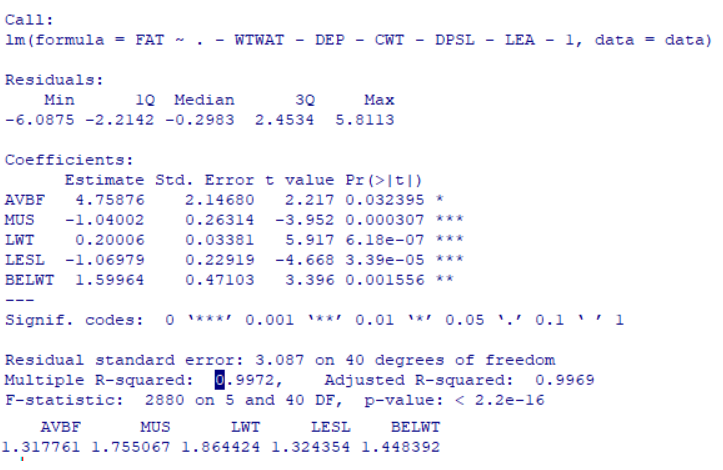
\includegraphics[scale = 0.80]{ExamenImG16.png}
 \caption{Resumen para modelo con las variables en la escala original. Eliminado \(\kis{CWT,DEP, WTWAT,DSPL, LEA}\) y el término de intercepto.}
\label{fig88}
\end{figure}

\textbf{d)} Para \(i \in \kis{AVBF,\hdots,BELWT}\) se define el vector columna de datos \(X_i\) como aquel que resulta de centrar el vector columna \(i\) y posteriormente escalar el vector resultante dividiendo por su longitud.\footnote{Entiéndase por longitud su norma euclideana.} Sea ahora \(\mathbf{X_{CE}} = \begin{pmatrix}  X_{AVBF} & \hdots & X_{BELWT}\end{pmatrix}\) 
ajustará\footnote{Note que \(\mathbf{X_{CE}}\) es exactamente la misma matriz que se definió en el inciso anterior} inicialmente el modelo
\begin{equation}\label{2.0}
 E[FAT_{i}| X_{AVBFi}, \hdots, X_{BELWTi}] =  \alpha + \delta_{1} X_{AVBF} + \hdots+ \delta_{10} X_{BELWTi}, \ i \in \kis{1, \hdots, 45}.
\end{equation}
 Sin embargo, de acuerdo a Hastie Tibsharani\footnote{Ver referencia 1, pp. 64.} considerando este modelo con las variables independientes centradas y escaladas se tiene que la estimación Ridge para el intercepto esta dada por \(\hat{\alpha} = \overline{FAT} = 55.082
\), y por ende es posible considerar de manera equivalente el modelo \eqref{1.2} y obtener mediante regresión Ridge las estimaciones para los coeficientes de dicho modelo utilizando la matriz de diseño \(\mathbf{X_{CE}}\)
\begin{equation}\label{2.2}
 E[FAT_{i} - \overline{FAT}| X_{iAVBF}, \hdots, X_{iBELWT}] = \delta_{1} X_{iAVBF} + \hdots+ \delta_{10} X_{iBELWT}, \ i \in \kis{1, \hdots, 45}.
\end{equation}
 De este modo además se cumplirá una de las condiciones estipuladas en el artículo de Hoerl (1975), es decir que la matriz de diseño \(\mathbf{X_{CE}}\) estará escalada de tal suerte que \(\mathbf{X_{CE}}'\mathbf{X_{CE}}\) sea una matriz de correlación. Ahora, de acuerdo al artículo de Hoerl (1975) una manera de estimar el valor del parámetro de sesgo \(\mathit{k}\) que resulte óptimo\footnote{En el sentido de que este \(\mathit{k}\) sea tal que el error cuadrático promedio que comete el estimador Ridge sea el mínimo posible.} es \begin{equation*}
    \mathit{k_h} = \frac{p \hat{\sigma}^2}{\hat{\delta}' \hat{\delta}} =0.08565412,
\end{equation*}
donde \(p\) es el número de parámetros en el modelo \eqref{2.2}, es decir \(p = 10\), \(\hat{\sigma}^2\) es una estimación de la varianza de los términos de error en el modelo \eqref{2.2}, la cual fue calculada usando la suma de cuadrados de los residuales del modelo \eqref{2.2} estimado por mínimos cuadrados y arrojó un valor de \(\hat{\sigma}^2 = 6.123102
\), y \(\hat{\delta}\) es el estimador de mínimos cuadrados para los coeficientes del modelo \eqref{1.2}.  Denote por \(\hat{\delta}_{(k_{h})}\) al vector de estimaciones Ridge de los coeficientes del modelo obtenido usando el parámetro de sesgo \(k_h\), calculado en el inciso \textbf{a)} de este ejercicio, entonces se tiene que
\begin{equation*}
    \hat{\delta}_{(k_{h})} = (\mathbf{X_{CE}}'\mathbf{X_{CE}} + k_h I_{p})^{-1}\mathbf{X_{CE}}'Y_{CE} =  \begin{pmatrix} -3.049124\\
  -7.406572\\
   -5.581604\\
   10.893713\\
    3.202395\\
    5.997023\\
 -6.552797\\
  -1.565149\\
  -6.561477\\
  6.4300717\end{pmatrix},
\end{equation*}
donde \(Y_{CE} = FAT - \overline{FAT}\). De este modo los valores ajustados por este modelo pueden escribirse como:
\begin{equation*}
 E[FAT_{i} - \overline{FAT}| X_{iAVBF}, \hdots, X_{iBELWT}] =  -3.049124 X_{iAVBF} + \hdots+  6.4300717X_{iBELWT}, \ i \in \kis{1, \hdots, 45}. 
\end{equation*}
Para esto modelo se obtuvo un \(R^2\) de 
\begin{equation*}
    R^2 = 1 - SS(RES)/SS(TOT) = 0.7972822. 
\end{equation*}
Llama la atención ya que es menor que el \(R^2\) del modelo completo con multicolinealidad, y es mucho menor al \(R^2\) del modelo propuesto en el inciso anterior. Pese a ello, el objetivo de la regresión Ridge fue logrado, ya que en la figura \ref{fig99} podemos ver los factores de inflación de la varianza para este modelo y todos ellos resultan menores a \(5\)
\begin{figure}[htb]
 \centering
 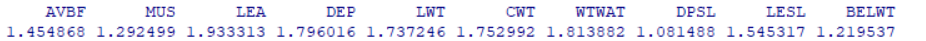
\includegraphics[scale = 0.80]{ExamenImG17.png}
 \caption{VIFS Modelo Ridge.}
\label{fig99}
\end{figure}
\end{solucion}
\end{document}
